\chapter{Background}
In this chapter, we introduce the Synchronous Message Exchange (SME) model and
briefly describe its origins, evolution, semantics, and implementations. The
design of SMEIL draws from the lessons learned throughout the brief time period
in which SME has existed. Here, we convey these insights to the
reader. Additionally, we motivate the need for custom hardware.

\section{Synchronous Message Exchange}
\label{sec:sme}

\subsection{The beginnings}
%The Synchronous Message Exchange model arose from a master thesis project 
The Synchronous Message Exchange model was conceived based on the experiences of
a masters thesis project \cite{Skaarup14} which attempted to generate a hardware
description from a model of a vector processor. The vector processor (described
in~\cite{rehr2013bpu}) was modeled with \gls{csp} using
PyCSP~\cite{bjorndalen2007pycsp}, a CSP library for Python. The initial
experiences using CSP for modeling the processor were promising. Especially the
process abstraction of CSP proved to be well suited for representing the
discrete components of a hardware design. Furthermore, the modularity
originating from the {\itshape shared-nothing} %\todo{Explain shared-nothing}
property of CSP was advantageous as it allowed seamlessly interchanging fine-
and coarse-grained implementations of the same discrete component.

\begin{figure}
  \centering
  \includegraphics[width=0.9\textwidth]{figures/clocked.pdf}
  \caption{In order to enforce synchronous communication semantics on a simple
    CSP network, a large amount of additional complexity is needed. Figure
    from~\cite{vinter2014synchronous}.}
  \label{fig:clocked}
\end{figure}

When the master thesis project, mentioned before, later attempted to convert the pure
CSP model to a hardware description, they found the CSP approach less apt.
% which later attempted to convert
% the CSP model to an actual hardware description found the pure CSP approach less
% apt.
Their experiences revealed a fundamental discrepancy between the data
propagation models of hardware and of CSP. In CSP, a process is free to
communicate at any time while in digital hardware, all communication is driven
forward synchronously by a clock.
% Enforcing globally synchronous communication using CSP is hard, since
% CSP is inherently asynchronous.
Thus, to accurately model hardware using CSP, this clock had to be emulated by
adding a single clock process with broadcasting channels to every process in the
network. Back-channels also had to be inserted for notifying
% from every process in the
% network to the clock process
the clock process when a process had finished running. Furthermore,
latch-processes had to be inserted into every channel going between processes,
ensuring that values were not propagated in the middle of a clock cycle. The
effect of adding these additional processes and channels is seen in
\Cref{fig:clocked}. Whenever the clock process emitted a signal, all processes
in the network would run. When the processes completed their run, the latch
processes ensured that values were propagated in the next cycle.
% When all processes had signaled a completed
% run, the clock would signal the latch processes in order to propagate the values
% of the network.

In the end, the thesis successfully managed to translate simple PyCSP networks
to VivadoC, a language for HLS. Despite this, the overall conclusion was that,
while CSP could be forced to adhere to globally synchronous semantics, the
networks required to do so were prohibitively complex. Furthermore, only a small
subset of the features in CSP was used to model the design. Particularly, a
concept central to CSP, \textit{external choice} which allows a process to
determine if it should run based on whether it received a message, was not found
to be applicable to hardware designs. However, not all was bad: As concluded by
the original vector-processor design work, the shared-nothing property of CSP
proved useful as the state of the network could only be altered by processes
communicating. This made it easy to compose networks without worrying about
inter-process dependencies.
% This made it simple to compose networks by making multiple
% instances of the same process.

Based on these experiences, the idea of using pure CSP as a hardware design tool
was discarded. In its place, a derived model, called SME, was conceived which
maintained the concepts of CSP that were found beneficial while adding a new,
globally synchronous, communication model~\cite{vinter2014synchronous}.

\subsection{The model}
The key concept of the SME model is the introduction of an implicit clock,
eliminating the complexity induced by forcing CSP to adhere to globally
synchronous message passing semantics.

% \todo{List properties}

% \begin{description}
% \item [Implicit clock]
% \item[..]
% \end{description}

% \subsubsection{SME components}
Building on its CSP roots, the fundamental unit in an SME network is the
{\itshape process}.  Networks are built by connecting processes through buses.
SME buses use the name ``bus'' instead of ``channel'', to reinforce the hardware
analogy and clarify its semantic equivalences with a physical signal bus found
in hardware. Furthermore, where channels in traditional CSP only support a
single value, a bus in SME is a bundle of individual channels connected to
processes as an entity.  This is also considered part of the hardware analogy
since a single signal path in hardware often consists of several individual
wires.

\subsubsection{Execution flow}
The SME concept of a ``clock cycle'' (\Cref{fig:smeclock}) goes through two
distinct phases. During the {\itshape compute phase} all processes are
run. During the {\itshape bus propagation} phase, values written to buses in the
current cycle are positioned to be read by processes in the following cycle.
% While the processes are running, the values of the reading ends of buses
% are kept constant. The {\itshape bus propagation} phase copies all values from
% the writing end of a bus to the reading end.

Each channel in a bus has separate reading- and writing-ends. During the compute
phase of a cycle, the reading-ends of channels are kept constant. The writing
end of a channel has a single-element overwriting buffer. Therefore, when a
process writes to a channel, the result is not immediately visible on the
reading end. The bus propagation phase copies all values from the reading-end to
the writing end. Thus, values written in cycle $c$, will be read in cycle
$c+1$. Another way to look at this is that, from the perspective of processes,
the values of all buses change simultaneously since value propagation happens
when the processes are not running.% \todo{Discuss process local state}

% This method for executing a clock cycle is the key to the SME model. Since the
% reading ends of a channel is kept constant during a cycle and only updated when
% no processes are running, the values of all channels simultaneously change from
% the point of view of the processes.

\begin{figure}
  \centering
\resizebox{.9\linewidth}{!}{
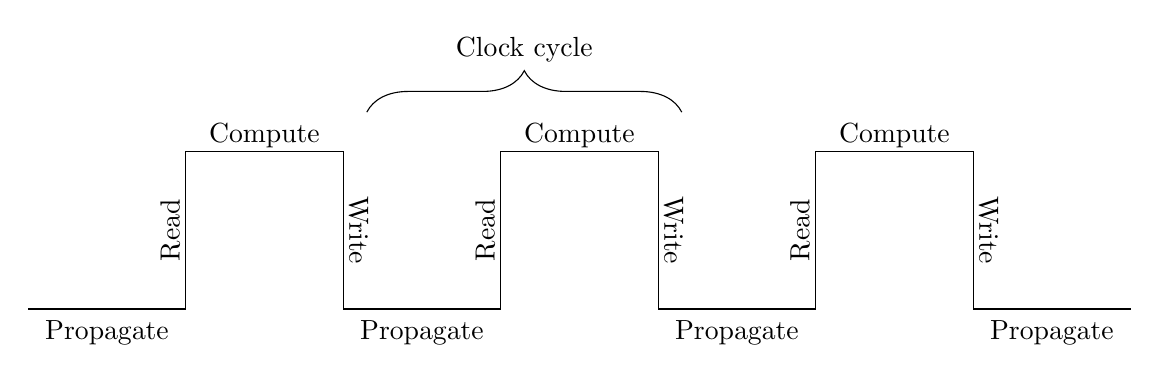
\begin{tikzpicture}
  \foreach \i in {0,4,8}
  \draw (\i,0) -- (\i+2,0) -- node [xshift=-0.2cm,rotate=90] {Read} (\i+2,2) -- node
  [yshift=0.2cm] {Compute}(\i+4,2) -- node [xshift=0.2cm,rotate=270] {Write} (\i+4,0);
  
  \draw (12,0) -- (14,0);
  \node [] at (13,-0.3) () {Propagate};

  \draw [decorate,decoration={brace,amplitude=15pt}] (4.3,2.5) -- (8.3,2.5) node
  [midway,yshift=0.8cm]{Clock cycle};

  \foreach \i in {0,4,8} {
  \node [] at (\i+1,-0.3) () {Propagate};
  % \node [blue] at (\i+3,-0.5) () {Run};
}

\end{tikzpicture}}
\caption{Illustration of the SME clock cycle concept.}
\label{fig:smeclock}
\end{figure}


% Even though you may already have realized the properties and components of the
% SME model, we give a more formal introduction here.

% A clock signal has four different states. Its either low, raising, high or
% falling. Conceptually, SME processes reads their input on the raising edge, then
% does computation, before writing the result of the communication.

% As referenced previously, the CSP concept of external choice was not found to be
% a good fit for hardware design, The key insight of the SME model is the concept
% of a \textit{hidden clock}


\subsubsection{An example}
\begin{figure}
  \centering
  \resizebox{.5\linewidth}{!}{
    \begin{tikzpicture}[font=\tiny,
      proc style/.style={circle,draw=black,align=center,text
        width=1cm,minimum size=1cm,align=center}
      ]
      \node[proc style] (id) {$=$};
      \node[below=0cm of id] (p1) {$P_1$};
      \node[proc style,right=2.5cm of id] (add) {$+1$};
      \node[below=0cm of add] (p2) {$P_2$};
      \draw[-{Latex[scale=1.6]}] (id) edge [bend left=30] node [above] {$b_2$} (add);
      \draw[-{Latex[scale=1.6]}] (add) edge [bend left=30] node [below] {$b_1$}
      (id);
    \end{tikzpicture}
    }
    \caption{A simple SME network consisting of two processes. One simply
      forwards the received value while the other increments it by one.}
  \label{fig:smeint}
\end{figure}

Even though the concepts of the SME model are uncomplicated, gaining an
intuition of value propagation governed by globally synchronous semantics is
harder. In an attempt to convey this intuition, we show an example of a simple
network, seen in \Cref{fig:smeint}. We return to a slight variation of this
example later, but for now, the network consists of two processes $P_1$ and $P_2$
and two buses connecting them, $b_1$ and $b_2$. In this network, a value is
passed around in a circular fashion. The process $P_1$ simply forwards the value
it receives while the $P_2$ process increments it by 1.\begin{figure}
  \centering
  \begin{tabular}{c|cccccccccc}
    %\toprule
    \diagbox[height=1.6em]{op}{c} & 1 & 2 & 3 & 4 & 5 & 6 & 7 & 8 & 9  \\\hline
    $P_1 \leftarrow b_1$          & 0 & 1 & 1 & 2 & 2 & 3 & 3 & 4 & 4  \\
    $P_1 \rightarrow b_2$         & 0 & 1 & 1 & 2 & 2 & 3 & 3 & 4 & 4  \\
    $P_2 \leftarrow b_2$          & 0 & 0 & 1 & 1 & 2 & 2 & 3 & 3 & 4  \\
    $P_2 \rightarrow b_1$         & 1 & 1 & 2 & 2 & 3 & 3 & 4 & 4 & 5  \\
    %\bottomrule
  \end{tabular}
  \caption{A table showing values read and written for every clock cycle of SME
    networks. Note that when we refer to a {\itshape trace} later, it is
    different from the table shown here. An SME trace file normally only
    contains the values of the reading ends of bus channels following every
    cycle.}
\label{tab:trace}
\end{figure}
In \Cref{tab:trace} we see the actual values read and written by every process
for every cycle. Note that before every cycle shown in the table, an implicit
bus propagation is run, driving forward the bus values. The arrows denote the
operation performed. A process can either {\itshape write into} or {\itshape
  read from} a bus. So, the operation $P_1 \rightarrow b_1$ means that $P_1$
writes to $b_1$. The reading-ends of all buses initially start out as 0. Thus,
in the first cycle, this value is read by both processes. In the second cycle,
we see the effect of the delayed value propagation: $P_2$ reads 0 again, even
though it wrote 1 in the previous cycle. Due to the single-cycle delay in value
propagation through a bus, the 0 read now in cycle $c$ was written by $P_1$ in
cycle $c-1$. This pattern continues and we show the first 9 cycles here. In
cycle 9, the value written by $P_2$ is 5.
% If value propagation
% was immediate


\begin{figure}
  \centering
  \resizebox{.9\linewidth}{!}{
    \begin{tikzpicture}[font=\tiny,
      rep style/.style={rectangle,draw=black,text width=1.5cm,minimum
        size=1cm,align=center},
      proc style/.style={circle,draw=black,align=center,text
        width=1cm,minimum size=1cm,align=center}
      ]
      \node[proc style] (impl) {SME model};
      \node[rep style,below=0.7cm of impl] (sim) {{\bfseries SME
        lib}\\Simulation\\Testing\\Code gen};
      \node[proc style,right=1cm of sim] (tb) {Test-bench};
      \node[proc style,above=0.5cm of tb] (trace) {CSV trace};
      \node[proc style,below=0.3cm of tb] (code) {VHDL Code};
      \node[gray,draw=gray,rep style,right=1cm of tb] (verifies) {Verifies};
      \node[proc style,left=1cm of code] (vendor) {Vendor tool};
      \node[rep style,left=1cm of vendor] (synth) {Synthesis};
      \node[proc style,above=1cm of synth] (fpga) {FPGA};


      \draw[-{Latex[scale=1.6]}] (impl) edge [] (sim);
      \draw[-{Latex[scale=1.6]}] (sim) edge [] (trace);
      \draw[-{Latex[scale=1.6]}] (sim) edge [] (tb);
      \draw[-{Latex[scale=1.6]}] (sim) edge [] (code);

     \draw[-{Latex[scale=1.6]}] (trace) edge [gray, bend left=20] (verifies);
     \draw[-{Latex[scale=1.6]}] (tb) edge [gray] (verifies);
     \draw[-{Latex[scale=1.6]}] (verifies) edge [gray, bend left=20] (code);

     \draw[-{Latex[scale=1.6]}] (code) edge [] (vendor);
     \draw[-{Latex[scale=1.6]}] (vendor) edge [] (synth);
     \draw[-{Latex[scale=1.6]}] (synth) edge [] (fpga);

    \end{tikzpicture}}
    \caption{A simplified overview of the steps taken from SME model to hardware
    implementation.}
  \label{fig:smeflow}
\end{figure}

\subsection{Using SME}
% The key advantage of SME is that a low-level hardware description may be
% generated form an SME network written in a high-level language.

The purpose of modeling a design in SME is to eventually convert it to an actual
hardware description. Regardless of which SME implementation is used (including
the one described in this thesis), the process goes through the same general
steps shown in \Cref{fig:smeflow}. The first step is to write the SME model and
related tests in a language with the required SME support. Then, this model is
read by the SME library which simulates the design and runs the related tests in
order to verify correctness. Three results are generated from the simulation: A
rendering of the SME design in an HDL (only VHDL has been used so far), a
test bench written in the HDL used for verifying the generated code and finally,
a \gls{csv}-file containing a value trace. The \gls{csv}-file is read by the
test bench which uses it as a source of input values to provide to the hardware
model and for checking that its output values are as expected. The generated HDL
code is then passed to a vendor tool for synthesis and eventual implementation
on hardware.

The present work only affects the stages up until passing the generated HDL to a
vendor tool.


% Regardless of
% which specific SME implementation is used, the workflow from SME model to
% hardware implementation generally follows the same steps seen in
% \Cref{fig:smeflow}. First, an SME implementation written in a general-purpose
% language is simulated, using a self-hosted simulator. The result of this
% simulation is a trace file containing the values of the reading-ends of buses
% for every cycle. The code is then translated to VHDL code and a test bench for
% testing the generated code. The test bench will, using the values of the trace
% file, cycle-for-cycle, test the generated code.

% The purpose of all ``model'' SME implementation is to eventually generate a
% hardware description.  Furthermore, verification of the generated VHDL code is simplified
% since also a test bench is generated. An overview of the process is shown in
% \Cref{fig:smeflow}. We show this, to give an understanding of what are the
% phases of a normal SME workflow. 



\subsection{Implementations}
A number of different library implementations of the SME model exist.

\subsubsection{\nth{1} PySME}
The initial implementation of SME was extremely simple: A mere 69 \gls{sloc} of
Python was all that was needed to create a library allowing Python programs to
be written following the SME model. This implementation was, of course, quite
rudimentary, however, it underlines a key advantage of the SME model. A person
can both understand the model and write an implementation from scratch in less
than a day.

\begin{widefigure}
  \centering
  \begin{minipage}{0.49\textwidth}
    \centering
    \includegraphics[width=.9\textwidth]{figures/add}
  \end{minipage}
  \begin{minipage}{0.49\textwidth}
    \centering
    \includegraphics[width=\textwidth]{figures/addnet}
  \end{minipage}
  \caption{An implementation of an adder (left) and a network using it (right)
    written using the original SME framework. Figure
    from~\cite{vinter2014synchronous}.}
  \label{fig:adder}
\end{widefigure}

An example of a network for adding together two values written using this SME
implementation is seen in \Cref{fig:adder}. As can be seen, this initial SME
version created connections between processes using {\itshape named
  channels}. So connecting a channel between two processes was done just by
referencing the same name as an input port and output port in the instances of
two different processes.


\subsubsection{\nth{2} PySME}
\label{sec:sme2}
After promising experiences with the first version of SME, a revision to the
model and its implementation was published~\cite{vinter2015bus}. This version
contained a number of changes, the most important being the abandonment of using
the aforementioned named channels for connecting processes. Instead, buses were
now considered first-class independent components of an SME
network. Furthermore, a bus was extended from being just a single channel to a
bundle of channels. Also included was a new top-level construct, named
\texttt{Network} used purely for defining buses and their connections to
processes. The adder shown in \Cref{fig:adder} using this version of SME is seen
in \Cref{fig:adder2}.

Modeling buses as active components of the network opened up a number of
possibilities, in particular generating the CSV trace-files mentioned above. A
disadvantage of this approach was that defining the connections of a complex
network quickly became unwieldy, as may already be visible from the very short
example in \Cref{fig:adder2}.

At this point, SME was only used for simulation and prototyping of hardware
designs. The completed prototypes were then manually translated to \gls{vhdl}
and verified using the trace-file generated by simulating the original SME
implementation. This was a tedious process, but it showed the viability of
translating SME models to a hardware description.


% After an initial experience with the first version of PySME the SME model was
% updated~ to include some changes that was deemed useful. The
% most noticeable change, was the abandonment of connecting processes through
% CSP-like singular channels in favor of Buses as described above. As buses were
% implemented as active participants in the network , it was now possible to use the buses
% to save a trace of the values flowing through the network. This allowed
% continuing verification when SME models was manually translated to VHDL,
% simplifying ensuring correctness of the generated code. Furthermore, this
% version of SME extended buses to be a collection of channels rather than just 

\begin{widefigure}
  \begin{multicols}{2}
    \small
\begin{lstlisting}[language=python]
from bSME import *

class Const(Function):
  # [..]

class Add(Function):
  def setup(self, args):
    self.cbus1, self.cbus2, self.out = args
    self.out["val"] = 0
  def run(self):
    self.out["val"] = self.cbus1["val"] +
                      self.cbus2["val"]

class Printer(Function):
  # [..]

class Adder(Network):
  def wire(self, args):
    self.constbus1 = Bus("Const1", "val")
    self.constbus2 = Bus("Const2", "val")
    self.resbus = Bus("Result", "val")
    self.c1 = Const("c1", [self.constbus1, 30])
    self.c2 = Const("c2", [self.constbus2, 5])
    self.add = Add("add", [self.constbus1,
                 self.constbus2,
                 self.resbus])
    self.printer = Printer("print",
                           [self.resbus])
Adder("Adder").clock(10)
\end{lstlisting}
  \end{multicols}
\caption{The adder shown in \Cref{fig:adder} implemented using the updated
  version of the SME framework.}
\label{fig:adder2}
\end{widefigure}

\subsubsection{C\# SME}
A C\# implementation of the new version of SME was also
created~\cite{skovhede2016building}. The primary change from the Python SME
implementations was the omission of a {\ttfamily Network}-like
construct. Instead, connections between a pair of processes were established if
they referenced the same bus. So instead of process instances being
parameterized with their connections, processes established connections
themselves by referencing buses. This proved to be a more comprehensible way of
building networks as the information about connections was spread out throughout
the program instead of being confined in a single class.  However, a shortcoming
of this approach was the one-to-one correspondence between process and bus
declarations and instances. This limitation was alleviated in later versions of
C\# SME library by the introduction of {\itshape scopes} which allowed several
instances of the same process to exist as long as they were defined in different
scopes.

This version of SME also facilitated automatic translation to \gls{vhdl}.

\subsubsection{\nth{3} PySME}
Based on the success of translating SME models written in C\# to VHDL, a project
was started to bring the same capability to the Python version of
SME~\cite{asheim2016vhdl}. The challenges of deriving static code from a dynamic
language were briefly mentioned in the introduction. Because of these
challenges, the previous PySME implementation was altered to require the
programmer to state her intentions more clearly. For example, in the \nth{2}
PySME, declaring a bus or instantiating a process could be done simply by
assigning a variable in the {\ttfamily wire} function of a network class. This
made analyzing the code difficult since the programmer's intention was not
clearly stated. Thus, an {\ttfamily add} method was added to the
\texttt{Network} class. This is the version of PySME used in the thesis.

\subsubsection{Conclusions}
The design of SMEIL draws heavily from the lessons learned by the different
approaches used by these SME implementations. 
% We have drawn two conclusions from the differing approaches used by C\# SME and
% the \nth{2} PySME which has influenced the design of SMEIL.
First of all, we concluded that requiring all buses and connections to be
declared in one place quickly become difficult to understand. The other is, that
it would be advantageous to associate process instances with bus instances to
avoid the same pitfall as the original C\# implementation. This is also helpful
when using SMEIL as an \gls{il} since buses and their connections translated
straightforwardly regardless of the originating implementation.


%%% Local Variables:
%%% mode: latex
%%% TeX-master: "../master"
%%% End:
